\section{Utilizzo dell'Applicazione}
\label{cap:utilizzo}
\subsection{Schermata principale}
All'avvio, la schermata di principale (Figura~\ref{fig:login}) permette di:
\begin{itemize}
    \item Effettuare il login con \textbf{Username} e \textbf{Password}, se già registrati.
    \item Registrare una nuova utenza (cliente o ristoratore).
    \item Accedere come ospite, fornendo delle coordinate geografiche per individuare i ristoranti più vicini.
\end{itemize}

\begin{figure}[H]
    \centering
    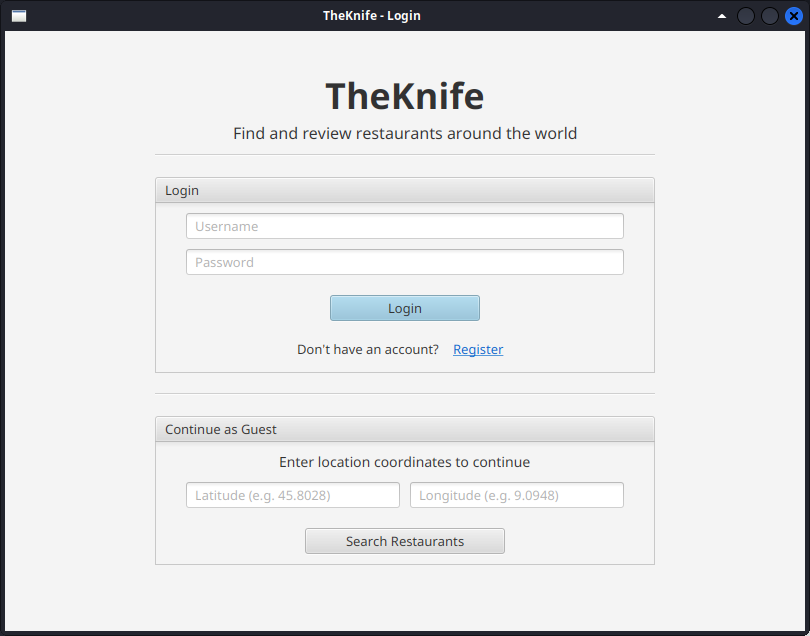
\includegraphics[width=0.8\textwidth]{images/login.png}
    \caption{Schermata principale}
    \label{fig:login}
\end{figure}

\subsection{Registrazione}
Per effettuare la Registrazione premere sul pulsante 
\emph{register} nella schermata principale 
(Figura~\ref{fig:login}).\\
Per effettuare correttamente la registrazione eseguire le 
seguenti azioni:
\begin{enumerate}
    \item Compilare tutti i campi.
    \item Selezionare il tipo di account: \emph{Cliente} o \emph{Ristoratore}.
    \item Premere sul pulsante \emph{Register} e completare la registrazione.
\end{enumerate}
\begin{figure}[H]
    \centering
    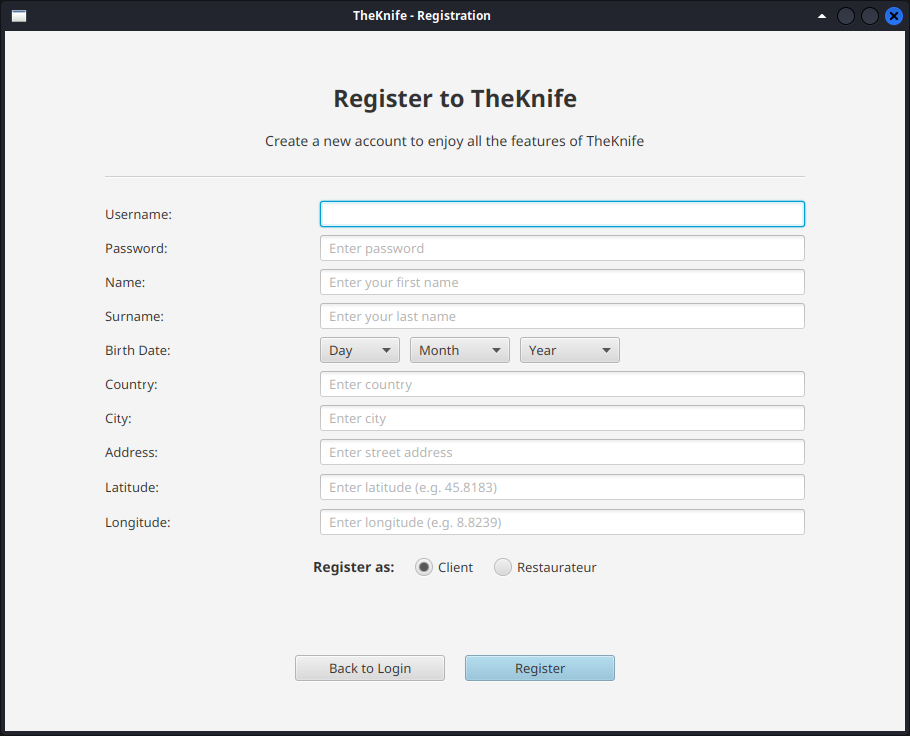
\includegraphics[width=0.8\textwidth]{images/registration.png}
    \caption{Registrazione}
    \label{fig:registration}
\end{figure}
Una volta terminata la registrazione, l'utente potrà effettuare il login con le credenziali scelte.
\paragraph{Sicurezza}
La password è salvata nel database cifrata con l'algoritmo di 
hashing \textit{Argon2} per garantirne la sicurezza, invitiamo 
tuttavia gli utenti a scegliere password che rispettino le 
comuni linee guida sulla complessità.

\paragraph{Esito della registrazione}
Una volta premuto il pulsante \emph{Register} comparirà un
messaggio indicante l'esito della registrazione.\\
Se la registrazione è andata a buon fine comparirà il seguente 
messaggio (Figura~\ref{fig:registration-ok}) e l'utente verrà reindirizzato alla schermata di 
login (Figura~\ref{fig:login}).
\begin{figure}[H]
    \centering
    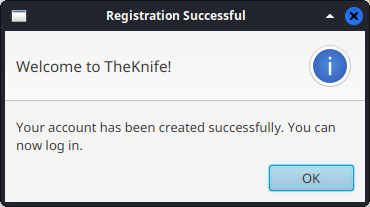
\includegraphics[width=0.8\textwidth]{images/r-ok.png}
    \caption{Registrazione andata a buon fine}
    \label{fig:registration-ok}
\end{figure}
Se la registrazione non è andata a buon fine comparirà 
un messaggio di errore (Figura~\ref{fig:registration-ko}) 
indicante il motivo dell'insuccesso della registrazione.
L'utente potrà correggere l'errore o scegliere di tornare alla
schermata di principale premendo il pulsante \emph{Back to Login}.
\begin{figure}[H]
    \centering
    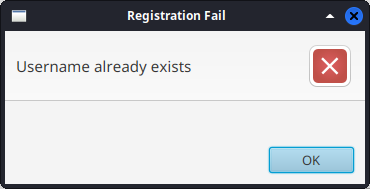
\includegraphics[width=0.8\textwidth]{images/r-ko.png}
    \caption{Registrazione fallita}
    \label{fig:registration-ko}
\end{figure}

\subsection{Ricerca}
Dopo il login, si accede alla schermata di ricerca (Figura~\ref{fig:search}).\\
La schermata mostra:
\begin{itemize}
    \item Pulsante di \emph{Logout}, in alto a destra, per tornare alla 
    schermata di login (Figura~\ref{fig:login})
    \item Le proprie coordinate geografiche 
    (latitudine e longitudine) in alto a sinistra
    \item Un pannello di ricerca per trovare ristoranti sulla sinistra
    \item Un pannello che mostra i ristoranti trovati dalla ricerca sulla destra
    \item \underline{Solo agli utenti registrati} il pulsante 
    \emph{My Area}, in alto a destra, alla sinistra del 
    pulsante \emph{Logout}, per poter accedere alla propria area personale
\end{itemize}
\begin{figure}[H]
    \centering
    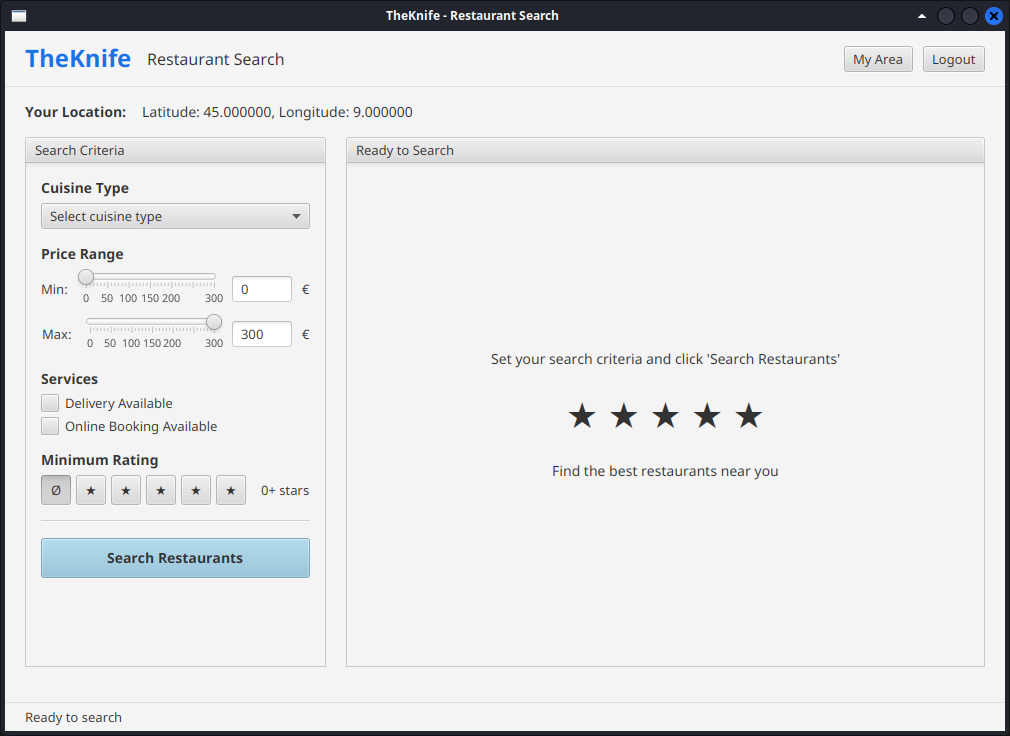
\includegraphics[width=0.8\textwidth]{images/search.png}
    \caption{Schermata di ricerca}
    \label{fig:search}
\end{figure}
Tramite il pannello di ricerca è possibile 
filtrare i ristoranti in base a:
\begin{itemize}
    \item Tipologia di cucina (es. italiana, cinese, messicana, ecc.)
    \item Fascia di prezzo (es. economico, medio, alto)
    \item Disponibilità di consegna a domicilio
    \item Disponibilità di prenotazione online
    \item Punteggio minimo (es. 1-5 stelle)
\end{itemize}
Una volta selezionati i filtri desiderati, 
premendo il pulsante \emph{Search Restaurant}, verrà
mostrata sulla destra la lista dei ristoranti più vicini 
che soddisfano i criteri di ricerca fino ad un massimo di 25.
\begin{figure}[H]
    \centering
    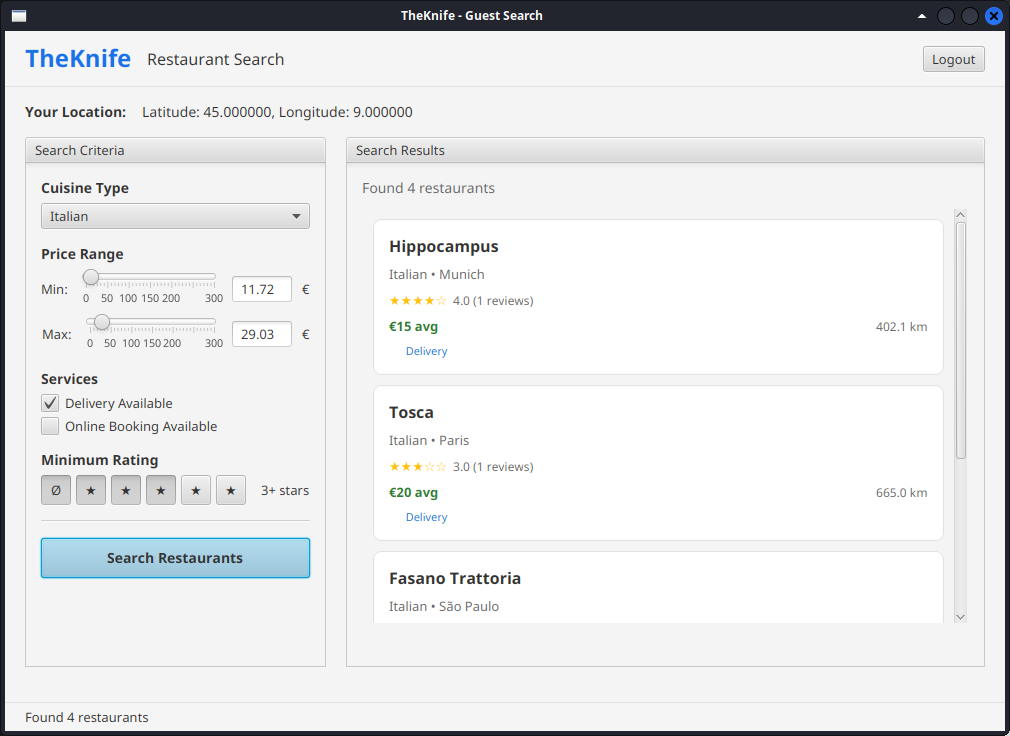
\includegraphics[width=0.8\textwidth]{images/search2.png}
    \caption{Ricerca dei ristoranti}
    \label{fig:search2}
\end{figure}

\subsection{Dettaglio del ristorante}
Selezionando un ristorante si accede alla pagina di dettaglio (Figura~\ref{fig:restaurant}), che include:
\begin{itemize}
    \item Nome del ristorante
    \item Tipologia di cucina
    \item Indirizzo completo del ristorante
    \item Coordinate geografiche (latitudine e longitudine)
    \item Distanza dall'utente
    \item Rating medio e numero di recensioni
    \item Prezzo medio
    \item Disponibilità di consegna a domicilio e prenotazione online
    \item Recensioni degli utenti
    \item Pulsante per aggiungere ai \emph{Preferiti} (solo utenti registrati).
    \item Pulsante per creare una nuova recensione (solo utenti registrati).
\end{itemize}

\begin{figure}[H]
    \centering
    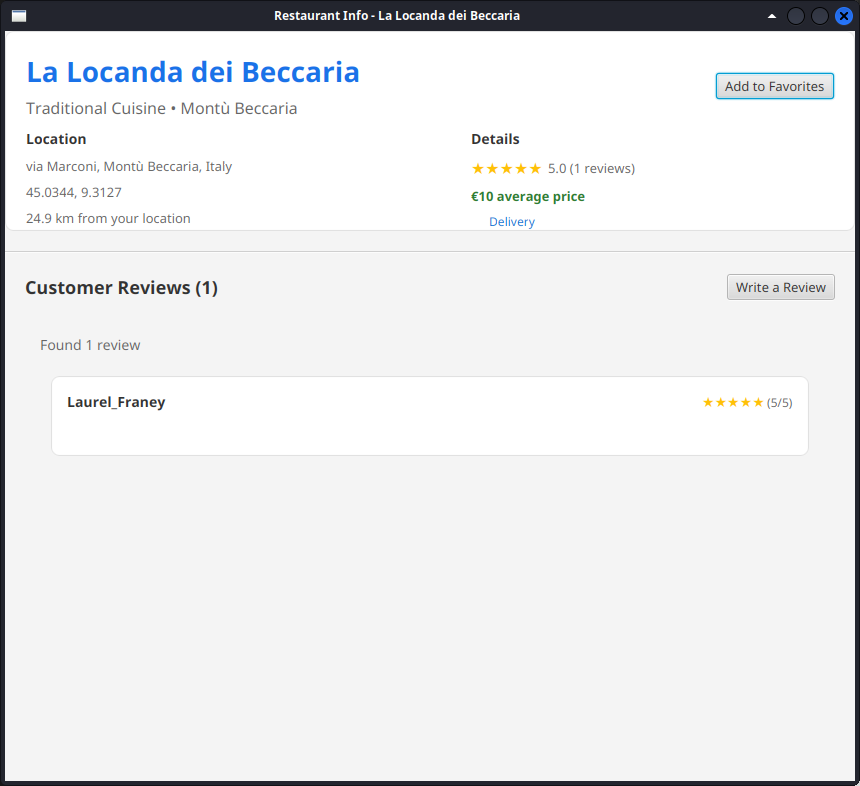
\includegraphics[width=0.8\textwidth]{images/restaurant.png}
    \caption{Pagina di dettaglio del ristorante}
    \label{fig:restaurant}
\end{figure}
